\begin{filecontents*}{mybib.bib}
@book{Sutton2018,
  added-at = {2019-07-13T10:11:53.000+0200},
  author = {Sutton, Richard S. and Barto, Andrew G.},
  biburl = {https://www.bibsonomy.org/bibtex/2f46601cf8b13d39d1378af0d79438b12/lanteunis},
  edition = {Second},
  interhash = {ac6b144aaec1819919a2fba9f705c852},
  intrahash = {f46601cf8b13d39d1378af0d79438b12},
  keywords = {},
  publisher = {The MIT Press},
  timestamp = {2019-07-13T10:11:53.000+0200},
  title = {Reinforcement Learning: An Introduction},
  url = {http://incompleteideas.net/book/the-book-2nd.html},
  year = {2018 }
}
\end{filecontents*}

\documentclass[10pt,a4paper]{article}
\usepackage[utf8]{inputenc}
\usepackage[top=1.25in, bottom=1.25in, left=.75in, right=.75in]{geometry}
\usepackage{amsmath}
\usepackage{algorithmicx}
\usepackage{algpseudocode}
\usepackage{algorithm2e}
\usepackage{amsfonts}
\usepackage{mathtools}
\usepackage{amssymb}
\usepackage{xcolor}
\usepackage{natbib}
\usepackage{bibentry}
\usepackage{float}
\usepackage{fancyhdr}
\usepackage{dsfont}
\usepackage{graphicx,caption}
\renewcommand{\familydefault}{\sfdefault}
\pagestyle{fancy}
\lhead{Exercise sheet \#3}
\nobibliography*
\DeclareMathOperator*{\argmax}{arg\,max}
\author{Johannes Ender}
\begin{document}
\clearpage
\setcounter{section}{2}
\section{Temporal Difference Learning}
\subsection*{35. Exercise 6.1 If V changes during the episode, then (6.6) only holds approximately; what would the difference be between the two sides? Let $V_t$ denote the array of state values used at time t in the TD error (6.5) and in the TD update (6.2). Redo the derivation above to determine the additional amount that must be added to the sum of TD errors in order to equal the Monte Carlo error. (page 121)}
\begin{align*}
G_t - V(S_t) &= R_{t+1} + \gamma G_{t+1} - [V(S_t) + \alpha[R_t + \gamma V(S_{t+1}) - V(S_t)]] + V(S_{t+1}) - \gamma V(S{S_{t+1}})\\
&= R_{t+1} + \gamma G_{t+1} - V(S_t) - \alpha R_t -\alpha \gamma V(S_{t+1}) + \alpha V(S_t) + \gamma V(S_{t+1}) - \gamma V(S_{t+1})\\
&= \delta_t + \gamma [G_{t+1} - V(S_{t+1})] - \alpha [R_t + \gamma V(S_{t+1}) - V(S_t)]\\
&= \sum_{k = t}^{T-1} \gamma^{k-t} \delta_k - \alpha [R_t + \gamma V(S_{t+1}) - V(S_t)] \\
&= \sum_{k = t}^{T-1} \gamma^{k-t} \delta_k  - \delta_t
\end{align*}
As at time step $t$, $V(S_t)$ is update with\\
\begin{align*}
V(S_t) = V(S_t) + \alpha \underbrace{[R_t + \gamma V(S_{t+1} - V(S_t)]}_{\delta_t}
\end{align*}
exactly $\alpha \delta_t$ is added; This is not done in the Monte Carlo algorithm, thus the MC error deviates at time step $t$ by this amount.
\subsection*{36. Exercise 6.8 Show that an action-value version of (6.6) holds for the action-value form of the TD error $\delta_t = R_{t+1} + \gamma Q(S_{t+1} , A_{t+1}) - Q(S_t , A_t )$, again assuming that the values don't change from step to step.}

\begin{align*}
G(S_t, A_t) - Q(S_t, A_t) &= R_{t+1} + \gamma G(S_{t+1}, A_{t+1}) - Q(S_t, A_t) \\
&= R_{t+1} + \gamma G(S_{t+1}, A_{t+1}) - Q(S_t, A_t) + \gamma Q(S_{t+1}, A_{t+1}) - \gamma Q(S_{t+1}, A_{t+1})\\
&= \delta_t + \gamma [G(S_{t+1}, A_{t+1}) - Q(S_{t+1}, A_{t+1})]\\
&= \delta_t + \gamma \delta_{t+1} + \gamma^2[G(S_{t+2}, A_{t+2}) - Q(S_{t+2}, A_{t+2})]\\
&= \sum_{k = t}^{T-1} \gamma ^{k-t}\delta_k
\end{align*}

\subsection*{37. Implementation Task: Windy Gridworld with King's Moves Exercise 6.9 Re-solve the windy gridworld assuming eight possible actions, including the diagonal moves, rather than the usual four. How much better can you do with the extra actions? Can you do even better by including a ninth action that causes no movement at all other than that caused by the wind? (page 130)}
Adding the possibility to also make diagonal moves enables the agent to reach the goal faster. In the figure below, one can see that towards the end of the learning episodes, on average it takes the agent 10 moves to reach the goal.
Allowing the agent to sit still and make no move at all, does not improve the results.
\begin{figure}[H]
\centering
\captionsetup{width=.5\linewidth}
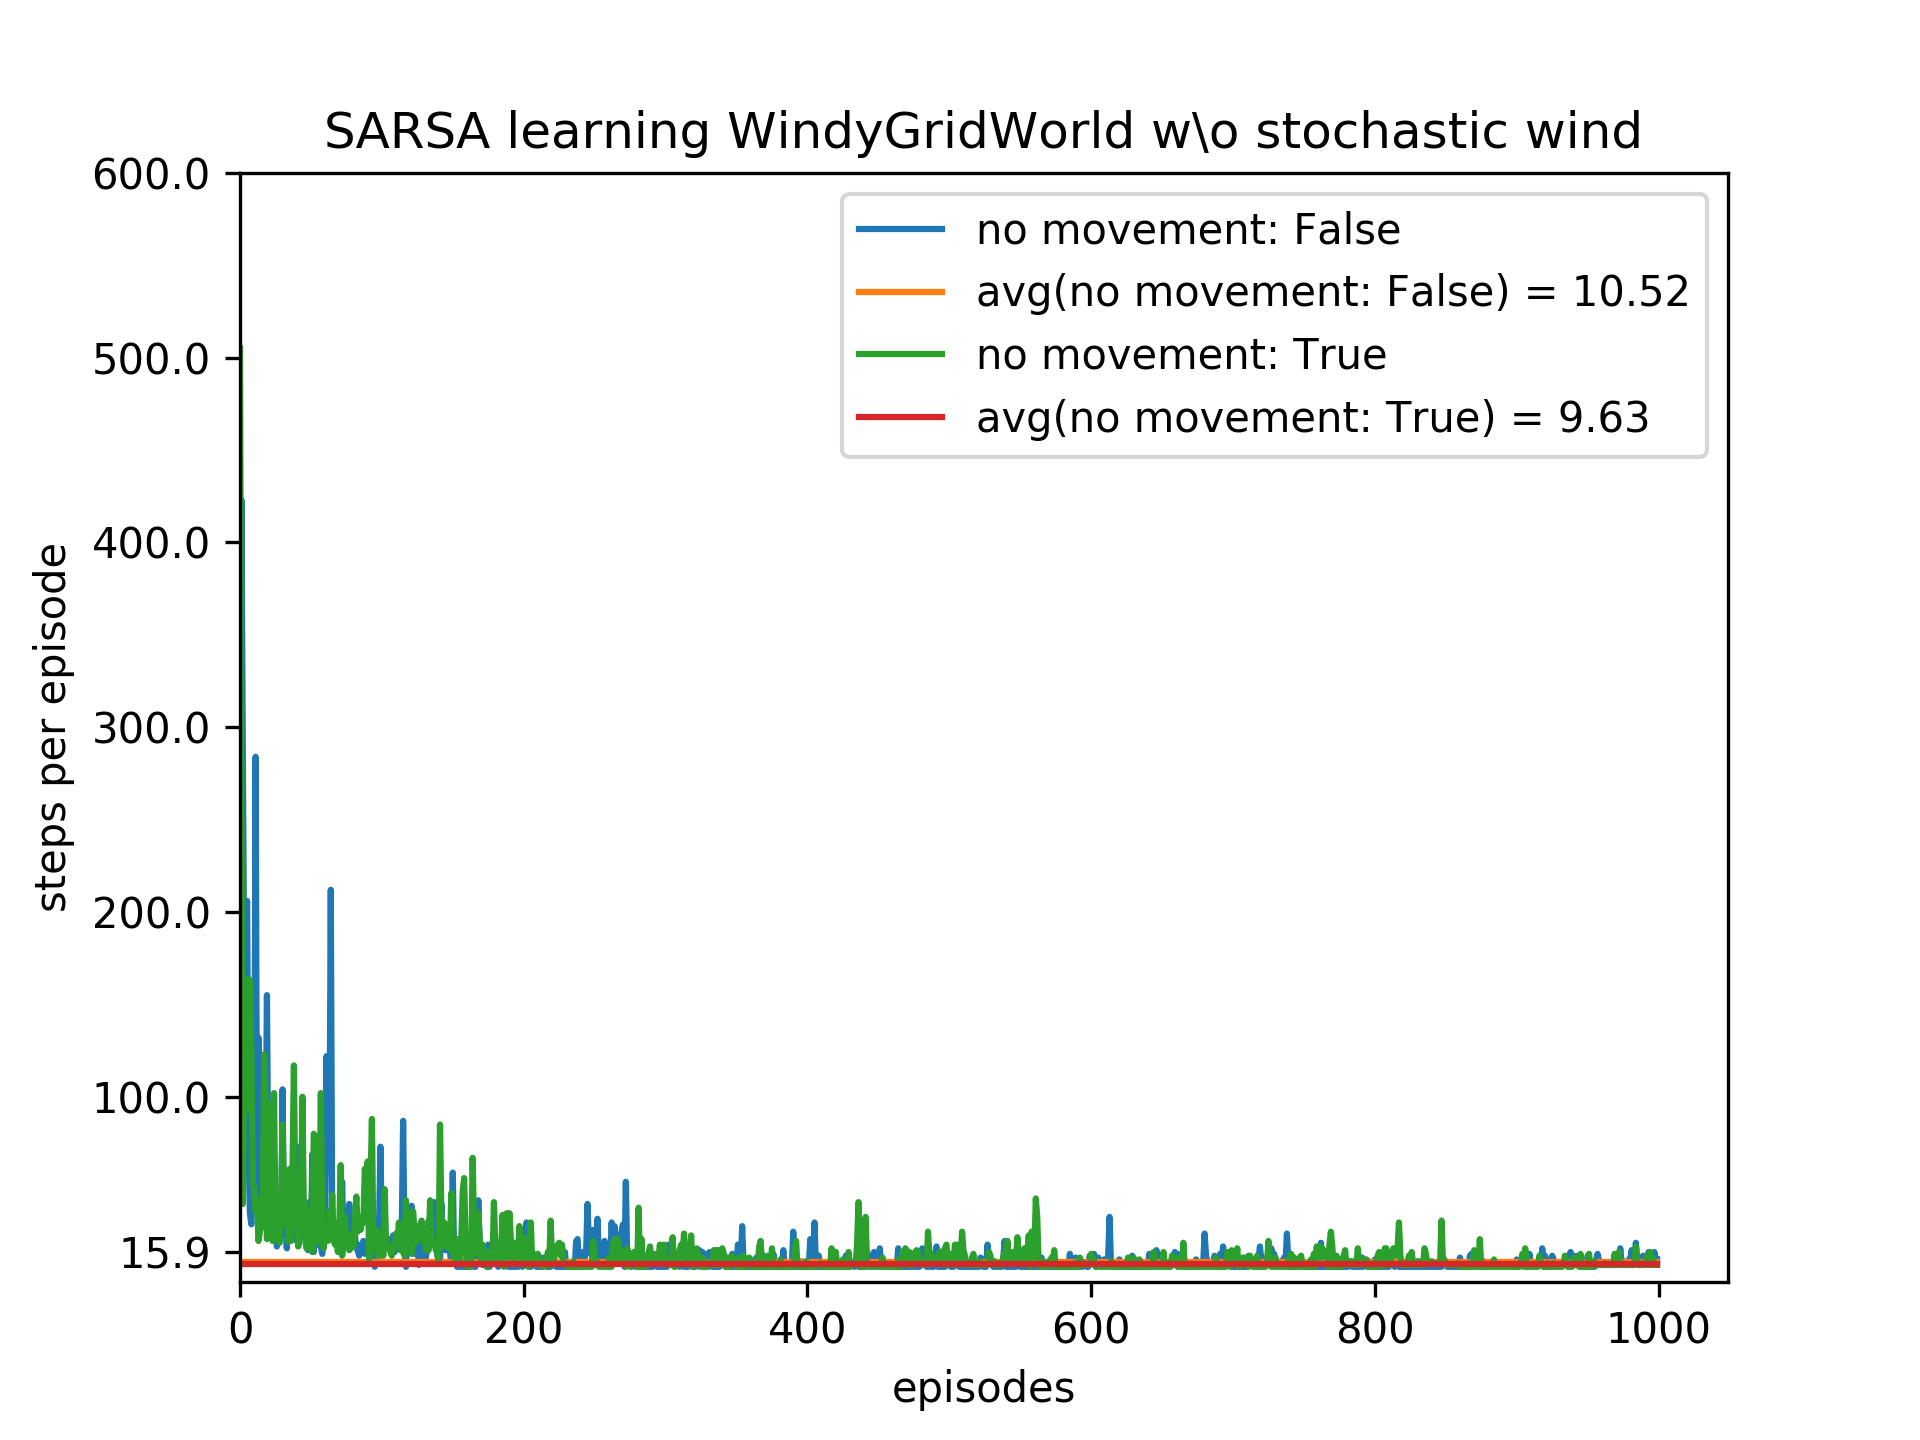
\includegraphics[width=.5\linewidth]{./WindyGridWorld_non_stochastic_wind.png}
\caption{Comparison of steps taken per episode for learning the windy gridworld problem using a SARSA agent. Averages are calculated over the last 100 episodes. Parameters: $\alpha = 0.5, \gamma = 1, \epsilon = 0.05$}
\end{figure}
Results were generated using the file \texttt{WindyGridWorld.py} and \texttt{utils.py}.
\subsection*{38. Implementation Task: Stochastic Wind Exercise 6.10 Re-solve the windy gridworld task with King's moves, assuming that the effect of the wind, if there is any, is stochastic, sometimes varying by 1 from the mean values given for each column. That is, a third of the time you move exactly according to these values, as in the previous exercise, but also a third of the time you move one cell above that, and another third of the time you move one cell below that. For example, if you are one cell to the right of the goal and you move left, then one-third of the time you move one cell above the goal, one-third of the time you move two cells above the goal, and one-third of the time you move to the goal.}
The figure below shows the results for the windy gridworld scenario with stochastic wind. One can see that towards the end of the learning process, the agent needs on 13 moves on average to reach the goal, i.e. around $\sim$30\% more.
Again, adding the possibility to sit still, does not improve or deteriorate the results.\\The small difference in the averages of the two scenarios simply arises from the specific random seed for this experiment, for other experiments with a different random seed, the averages are the same or the average for the 'no movement: True' scenario is higher.
\begin{figure}[H]
\centering
\captionsetup{width=.5\linewidth}
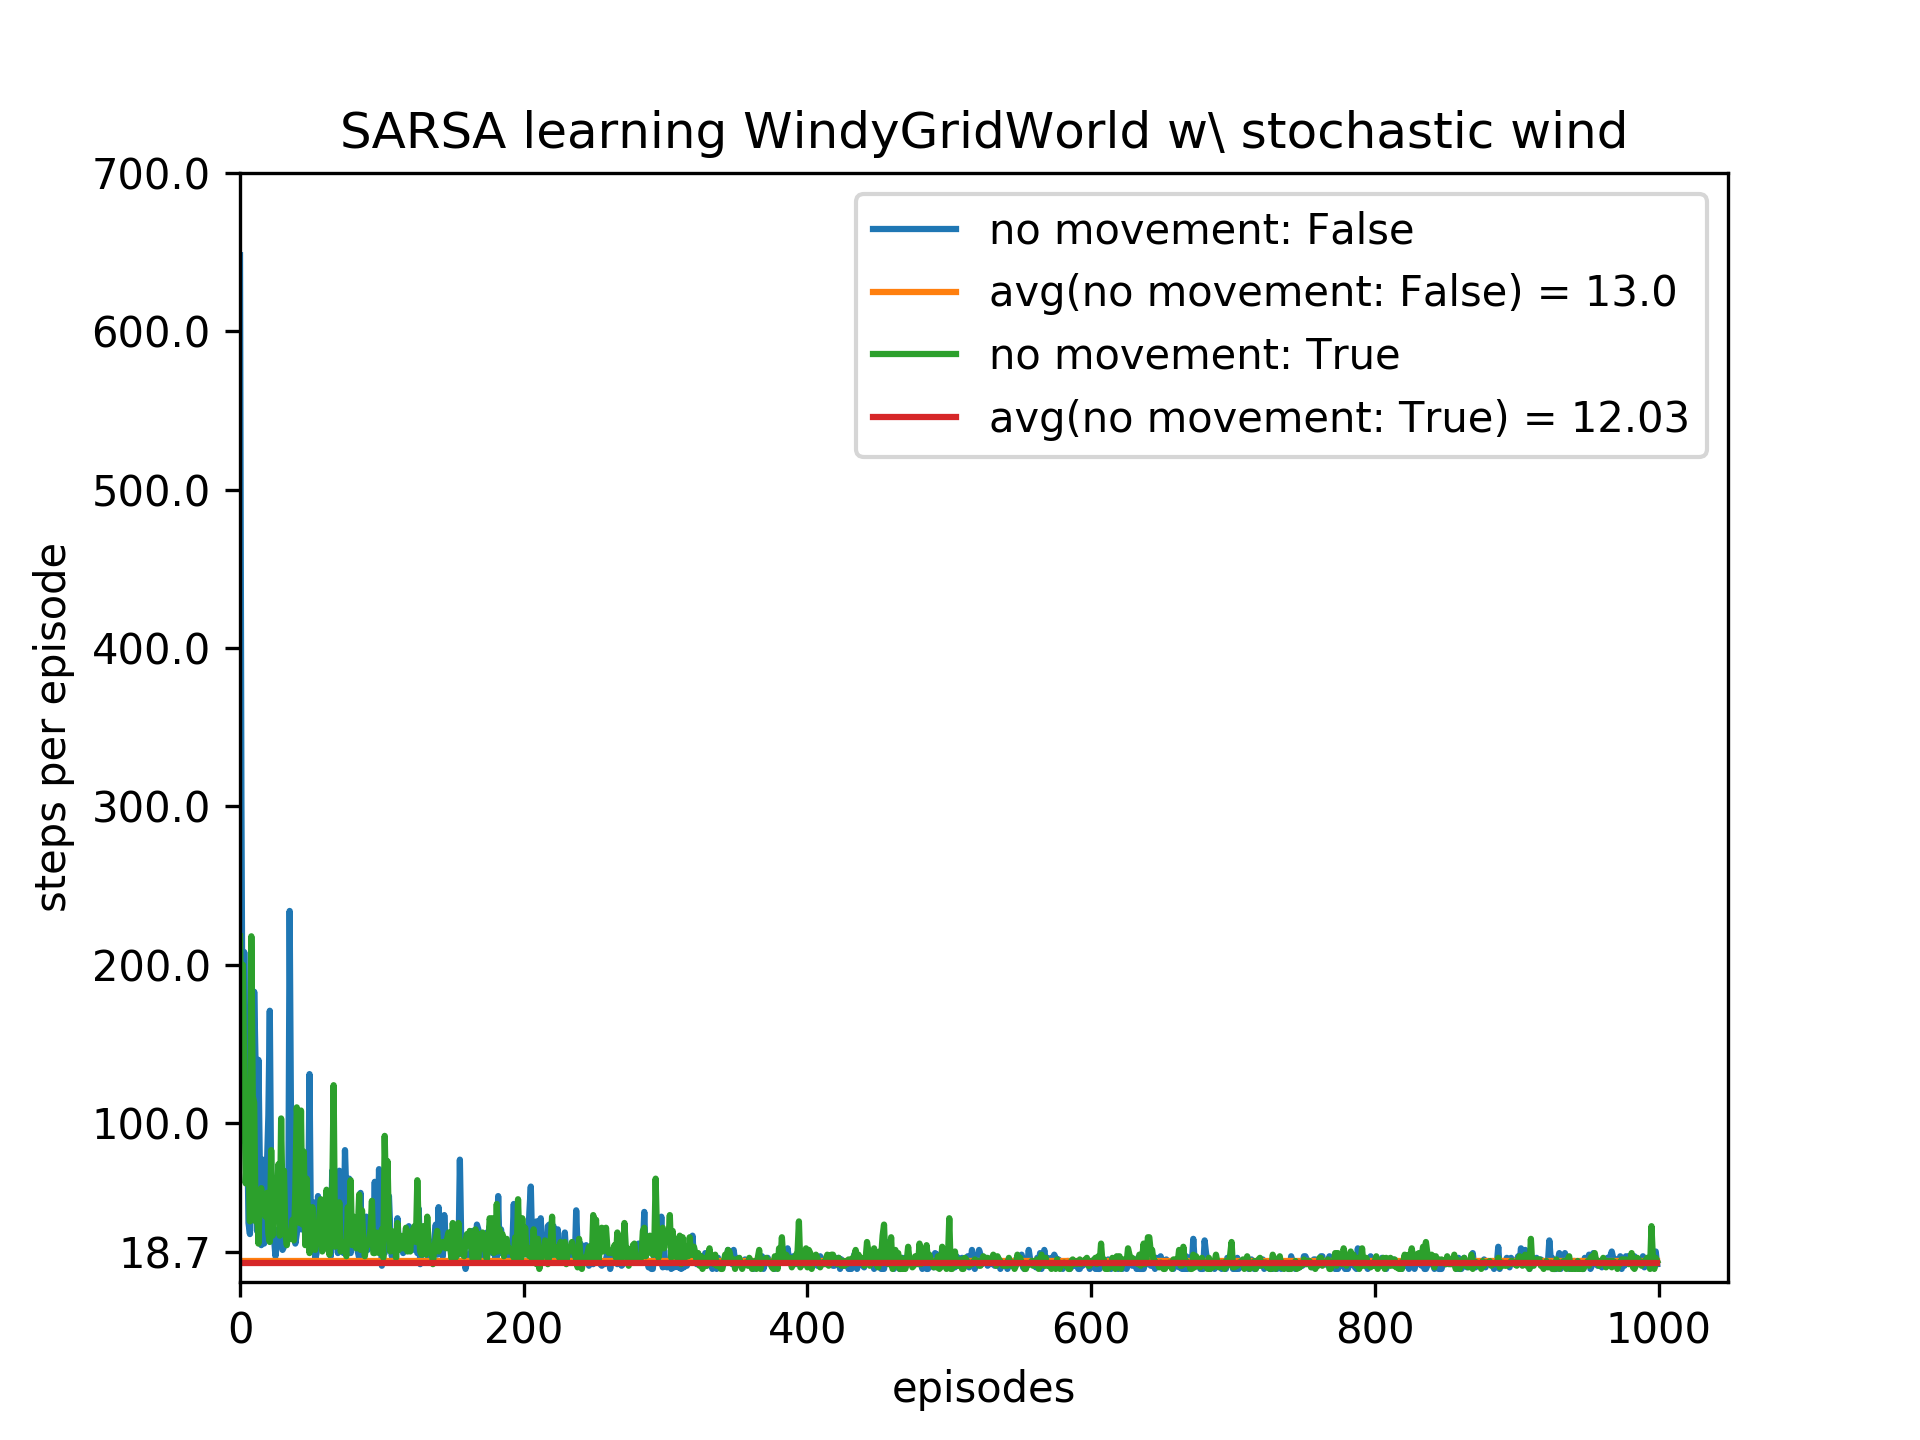
\includegraphics[width=.5\linewidth]{./WindyGridWorld_stochastic_wind.png}
\caption{Comparison of steps taken per episode for learning the windy gridworld problem with stochastic wind using a SARSA agent. Averages are calculated over the last 100 episodes. Parameters: $\alpha = 0.5, \gamma = 1, \epsilon = 0.05$}
\end{figure}
Results were generated using the file \texttt{WindyGridWorld.py} and \texttt{utils.py}.
\subsection*{39. Exercise 6.11 Why is Q-learning considered an off-policy control method?}
In Q-learning, the decision which action to take is made based on some ($\epsilon$-greedy) policy, while in the update of the action-value function, $\underset{a}{\operatorname{max}}Q(S', a)$ is used, i.e. it is absolutely greedy.

\subsection*{40. Exercise 6.12 Suppose action selection is greedy. Is Q-learning then exactly the same algorithm as Sarsa? Will they make exactly the same action selections and weight updates?}
No, even if action selection is greedy they are not the same.\\
Sarsa performs the action selection for the next time step before updating the action-value function, while Q-learning uses the already updated action-value function.

\subsection*{41. Exercise 6.13 What are the update equations for Double Expected Sarsa with an $\epsilon$-greedy target policy?}
With e.g. probability $0.5$ use this update:
\begin{align*}
Q_1(S, A) &= Q_1(S, A) + \alpha [R' + \gamma \underset{a}{\sum}\pi_2(a \mid S') Q_2(S', a) - Q_1(S, A)]
\end{align*}
otherwise use the same update with the indices reversed. $\pi_2$ is an $\epsilon$-greedy policy w.r.t. $Q_2$.

\newpage
\section*{n-step Bootstrapping}
\subsection*{42. Exercise 7.1 In Chapter 6 we noted that the Monte Carlo error can be written as the sum of TD errors (6.6) if the value estimates don't change from step to step. Show that the n-step error used in (7.2) can also be written as a sum TD errors (again if the value estimates don't change) generalizing the earlier result. (page 143)}

\subsection*{43. Implementation Task: n-step Algorithm Exercise 7.2 With an n-step method, the value estimates do change from step to step, so an algorithm that used the sum of TD errors (see previous exercise) in place of the error in (7.2) would actually be a slightly different algorithm. Would it be a better algorithm or a worse one? Devise and program a small experiment to answer this question empirically.}

\newpage
\section*{Planning and Learning}
\subsection*{44. Implementation Task: n-step Algorithm vs Planning\\Try to reproduce Figure 8.2 on page 165. Then apply a multi-step algorithm to this problem. What does the performance comparison look like?}
From the figure below, one can see that the multi-step Sarsa algorithm cannot compete with the planning algorithms.
\begin{figure}[H]
\centering
\captionsetup{width=.5\linewidth}
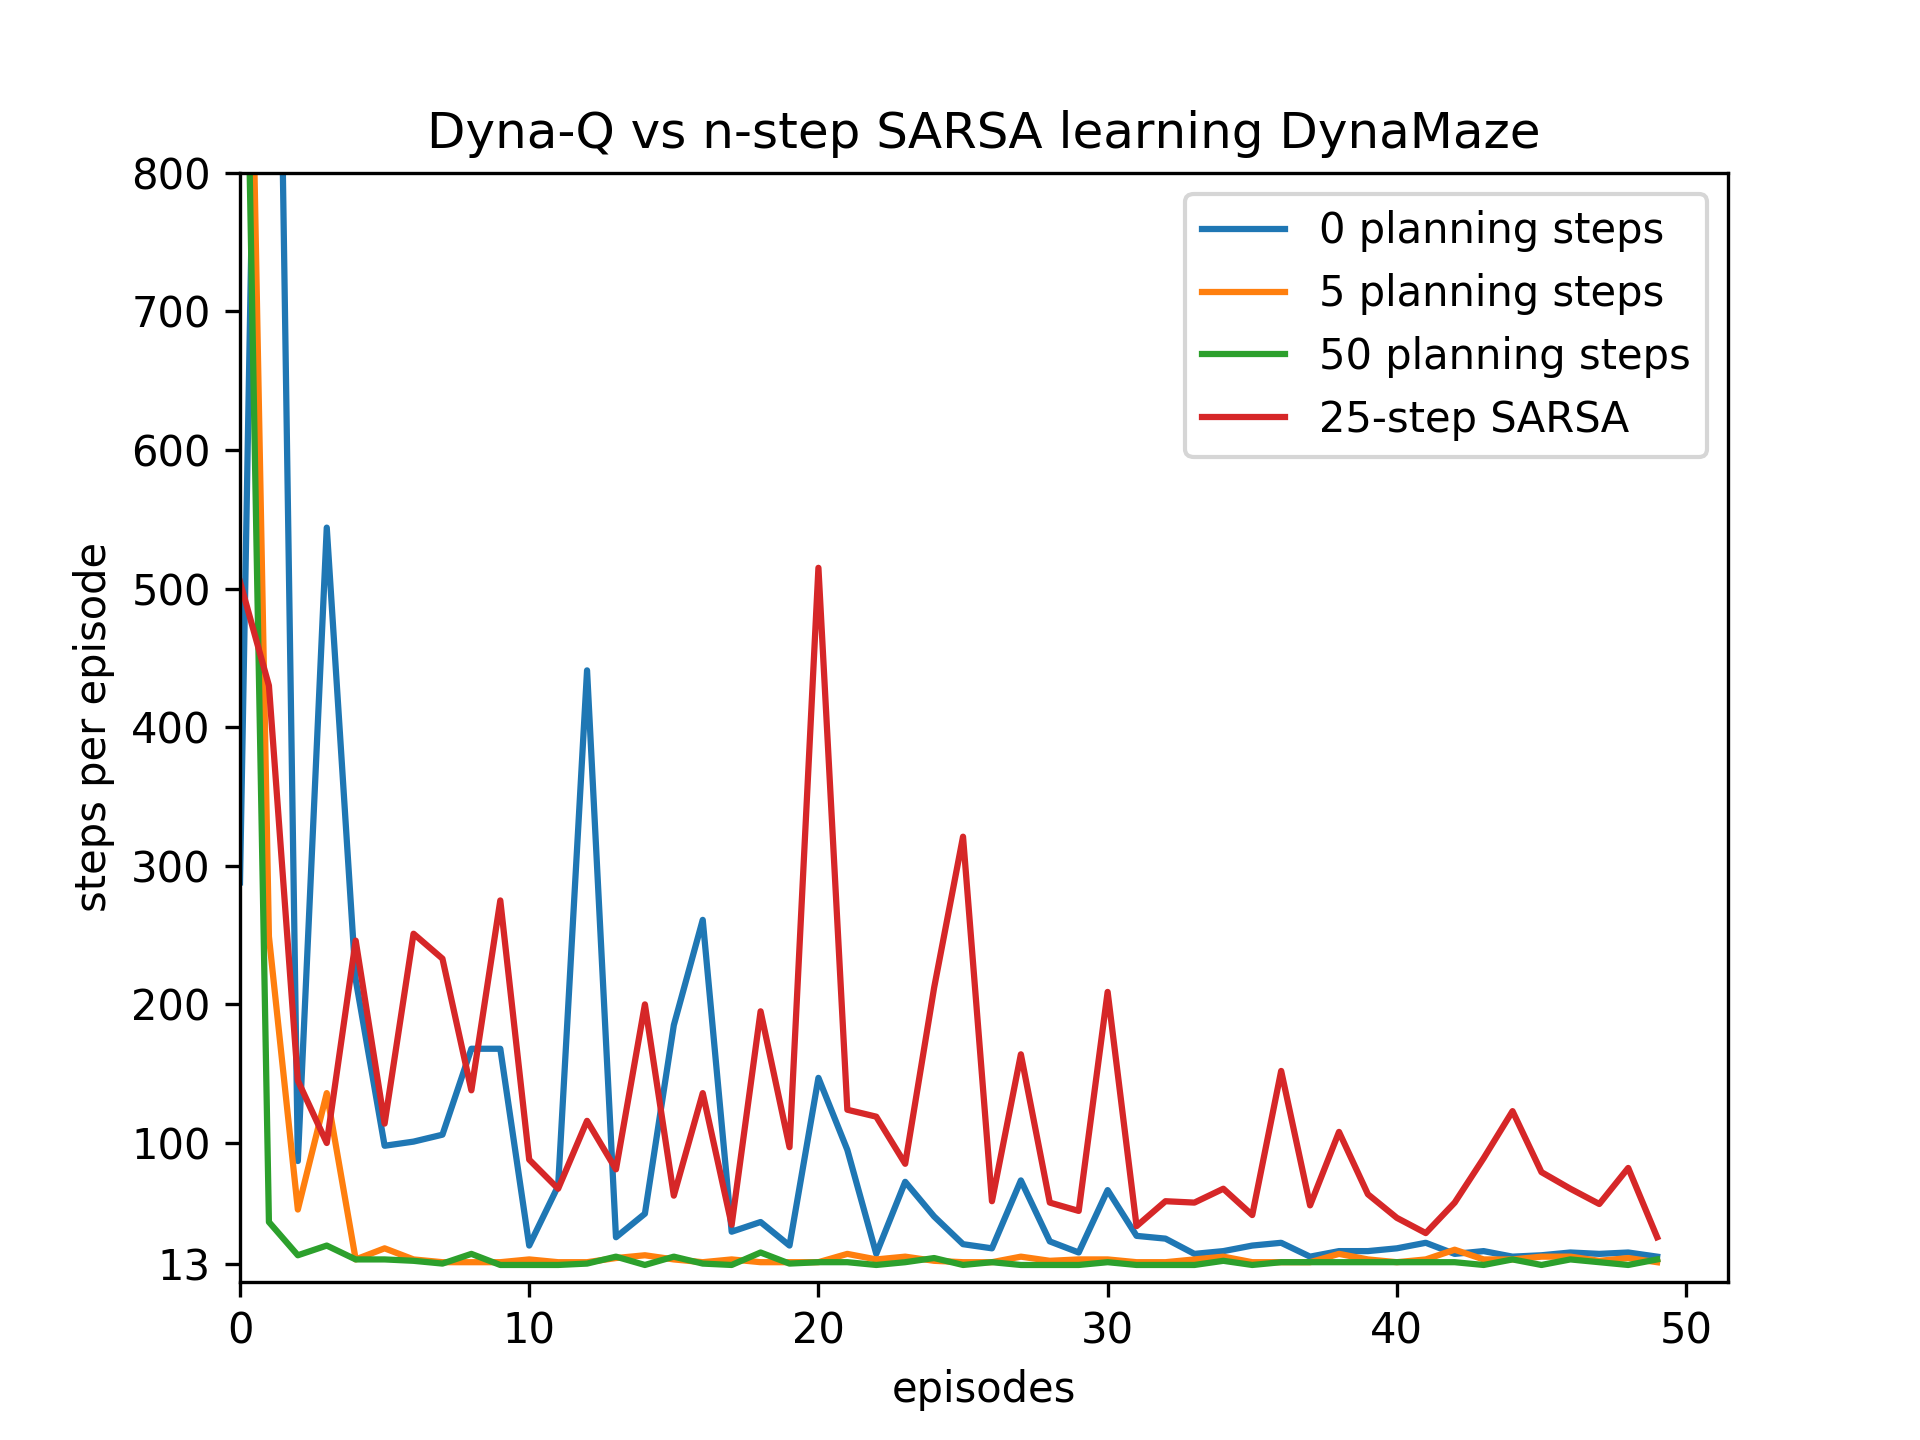
\includegraphics[width=.5\linewidth]{./planning_vs_nstep.png}
\caption{Comparison of planning Dyna-Q agents with different numbers of planning steps with an n-step SARSA agent. Parameters: $\alpha = 0.5, \gamma = 1, \epsilon = 0.05$}
\end{figure}
Results were generated using the file \texttt{DynaQ.py, nStepSARSA.py} and \texttt{utils.py}.

\subsection*{45. Exercise 8.1 The nonplanning method looks particularly poor in Figure 8.3 because it is a one-step method; a method using multi-step bootstrapping would do better. Do you think one of the multi-step bootstrapping methods from Chapter 7 could do as well as the Dyna method? Explain why or why not.}
Although multi-step methods would do better than a one-step method, they could not compete with the Dyna method.\\
The Dyna method makes many more updates to the current estimate of the action-value function and is thus more sample efficient.
\newpage
\bibliographystyle{plainnat}
\bibliography{mybib}
\end{document}